\chapter{Literature Review and Related Work}
\label{chap:relatedworks}

Generative AI has seen rapid advancements, particularly in video synthesis and manipulation. 
However, as AI-generated content becomes more sophisticated, concerns over deepfake misuse, copyright violations, 
and data exploitation has risen. Several existing tools attempt to address these challenges, 
but they focus primarily on static image protection rather than video poisoning.

\clearpage

\section{Competitor Analysis}
\label{section:competitor-analysis}

\begin{figure}[h]
    \centering
    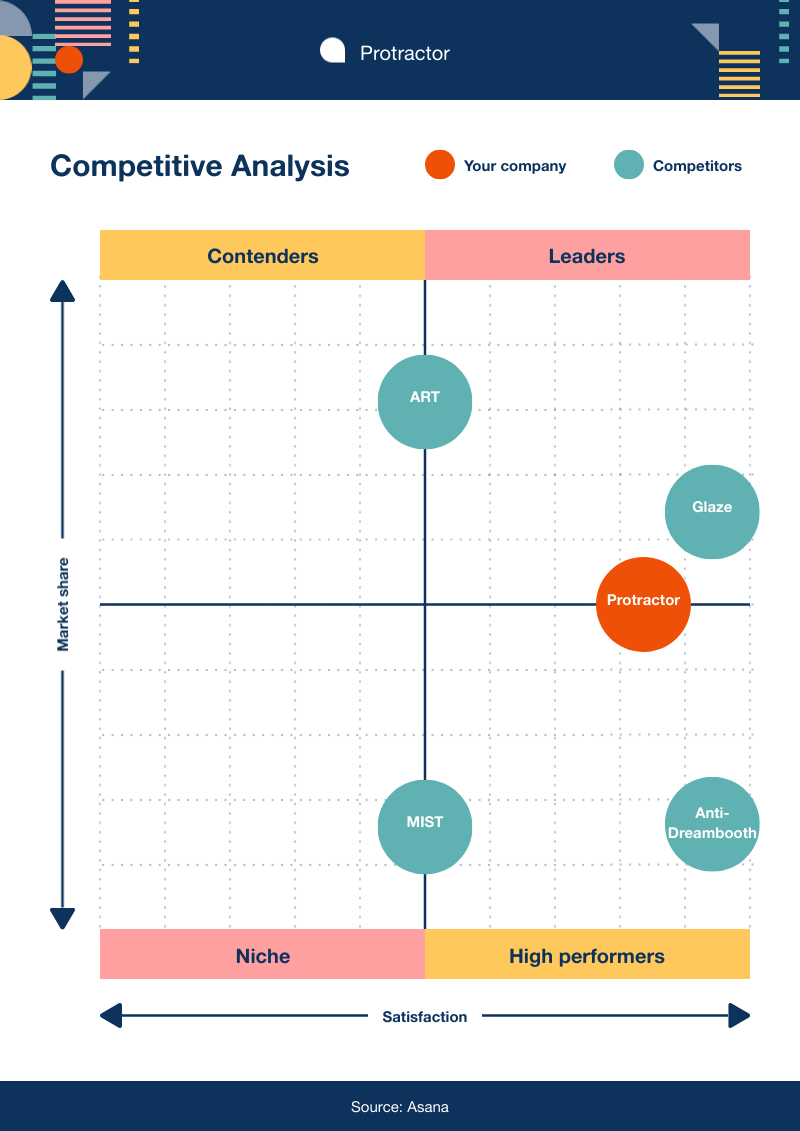
\includegraphics[width=0.5\textwidth]{chapter_2/competitors/competitive-analysis.png}
    \caption{Competitive Landscape}

\end{figure}

Because there are currently no poisoning processors for videos, our current competitor would be static image poisoning processors, in a scenario where they extract the video's graphics frame by frame, and poison each of them as a static image, and then reassemble them back as a video.

    The goal of the software is to protect the video from AI training by data poisoning method Adversarial attack; to break AI's accuracy by adding information to the data that is imperceptible to the human eye.

    \clearpage

    \begin{enumerate}
        \item Glaze
        
        \par Glaze is a tool that applies adversarial perturbations to digital artwork to prevent AI from learning its style. It modifies the image in a way that disrupts AI training while keeping the visual impact minimal to the human eye.
        Like other competitors, it only targets static images. Their poisoning method is less effective against AI due to video denoiser Autoencoder using more techniques such as temporal Consistency or attention seeking transformer methods which makes perturbations for static images less effective, and takes too long to be implemented Frame by frame, as a 10 minutes long video with 30 fps could take a minimum of 8 hours.
        
        \item MIST
        \par MIST is another adversarial tool designed to mislead AI models into misinterpreting images, effectively reducing the accuracy of AI-based recognition and training systems. It faces the same challenges as Glaze for its implementation in video poisoning.

        
        \item Anti-Dreambooth
        \begin{figure}[h]
            \centering
            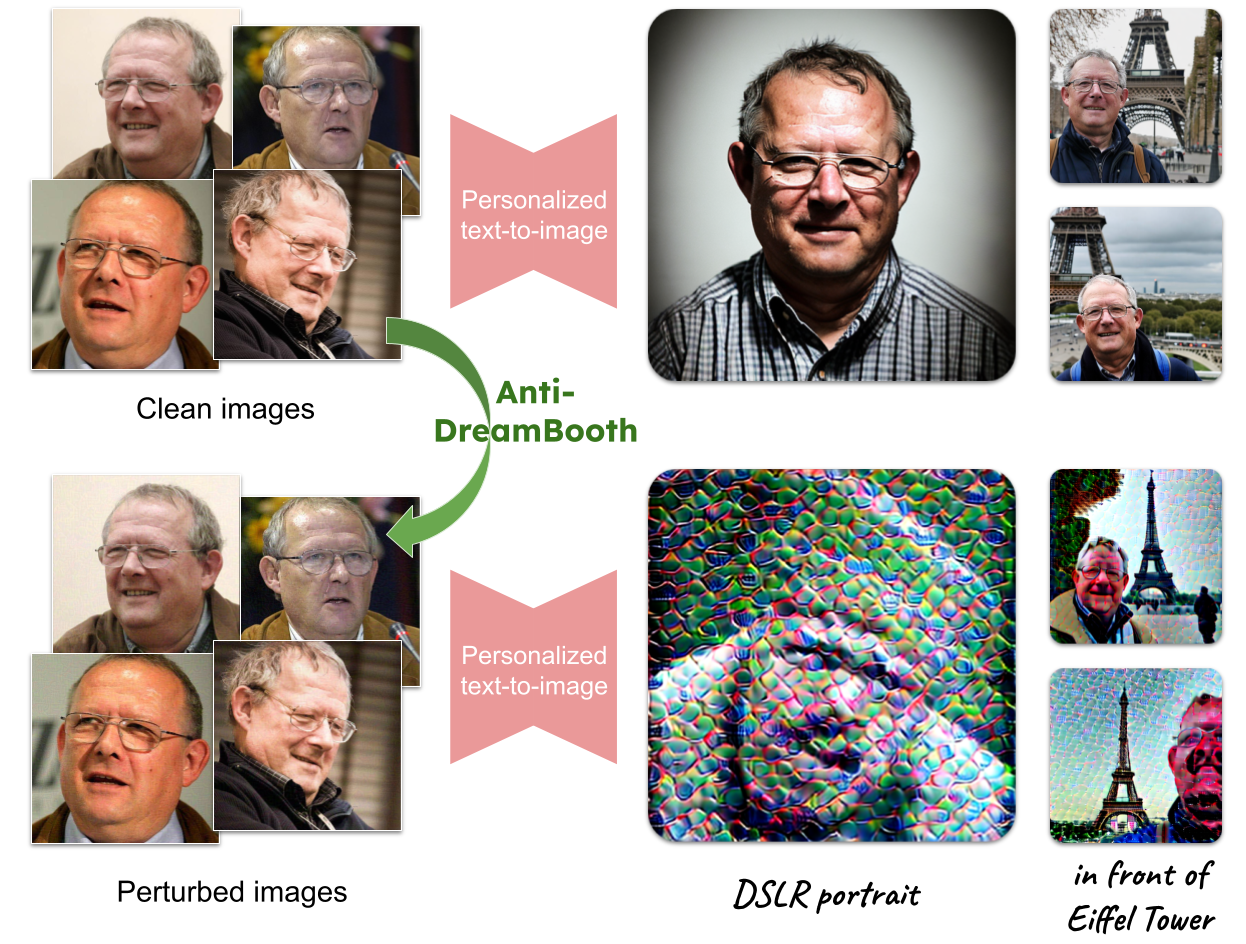
\includegraphics[width=0.5\textwidth]{chapter_2/competitors/Anti-DreamBooth_sample.jpg}
            \caption{Anti-DreamBooth sample demonstration}
        
        \end{figure}
        \par Anti-Dreambooth targets models that fine-tune on small datasets, introducing noise patterns that degrade the ability of AI to generate imitative outputs. It faces the same challenges as Glaze for its implementation in video poisoning.

        
        \item ART : Adversarial Robustness toolbox
        \par The Adversarial Robustness Toolbox (ART) is a broader security-focused framework that provides methods for generating adversarial attacks and defenses against AI-based recognition.
        There are currently no video perturbation methods implemented yet.

        
    \end{enumerate}

\section{Literature Review}
\label{section:literature-review}

\begin{enumerate}
    \item stAdv
        
    \par stAdv : Spatially Transformed Adversarial Attack
    \begin{figure}[h]
        \centering
        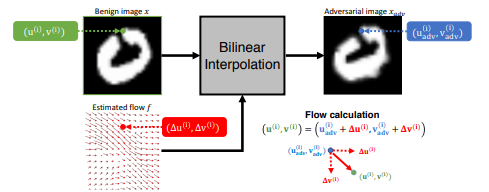
\includegraphics[width=0.5\textwidth]{chapter_2/research/stAdv.png}
        \caption{Explanation of how perturbation is added}
    
    \end{figure}

    stAdv is a type of adversarial attack based on local geometric transformations.
    \begin{figure}[h]
        \centering
        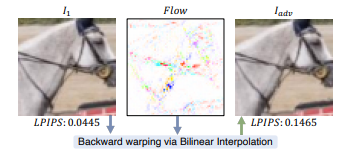
\includegraphics[width=0.5\textwidth]{chapter_2/research/stAdv_with_LPIPS.png}
        \caption{Explanation of how perturbation is added with LPIPS to measure perceptual similarity between the original and the poisoned output}
    
    \end{figure}

    It has been shown by CAM attention visualization to shift the focal point of attention away from the original's, and proven to be stronger than FGSM and C\&W method
    \begin{figure}[h]
        \centering
        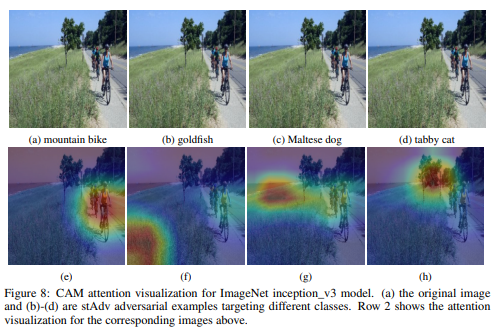
\includegraphics[width=0.5\textwidth]{chapter_2/research/stAdv_results.png}
        \caption{CAM attention results after image had been poisoned}
    
    \end{figure}
    \begin{figure}[h]
        \centering
        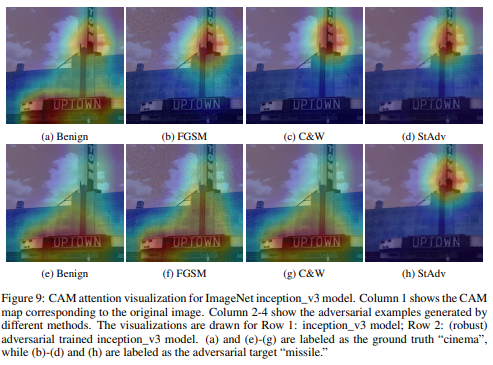
\includegraphics[width=0.5\textwidth]{chapter_2/research/stAdv_against_other.png}
        \caption{CAM attention results of stAdv compared to FGSM and C\&W perturbation where Benign is the control sample}
    
    \end{figure}

    \clearpage

    \item BTC-UAP
    \begin{figure}[h]
        \centering
        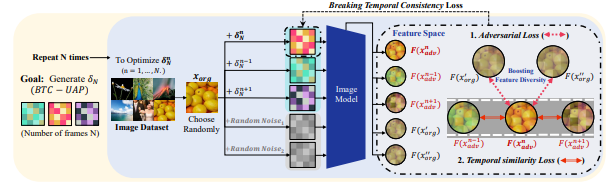
\includegraphics[width=0.5\textwidth]{chapter_2/research/BTC-UAP.png}
        \caption{BTC-UAP poisoning logic}
    
    \end{figure}
    \par BTC-UAP : Breaking Temporal Consistency - Universal Adversarial Perturbation

    BTC-UAP is a technique that changes videos in a way that confuses AI, making it harder to recognize patterns. This is crucial in staying subtle enough so the output image stays perceptually similar to human and not easily removable by Video Denoising Autoencoder, but strong enough to break AI's Temporal Consistency after they trained on data poisoned with BTC-UAP.

    \begin{figure}[h]
        \centering
        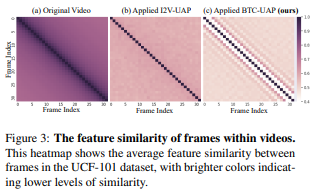
\includegraphics[width=0.5\textwidth]{chapter_2/research/Temporal_consistency_results.png}
        \caption{Heatmap of Temporal Consistency; darker means better Consistency}
    
    \end{figure}

    Here it is demonstrated that the Temporal Consistency of BTC-UAP is the best perturbation that breaks AI’s performance worst, while the output is still perceptually identical to the original video input.
    
\end{enumerate}


To optimize our software and be a reliable data security tool, This project will be built upon various researches like these to ensure their effectiveness against bad actors from using the ever-evolving State-of-the-Art Generative AIs as a tool to exploit user's data.
